\documentclass[tikz,border=8pt]{standalone}
% Shared look for every TikZ diagram. Load with \input{../../tools/tikz-style.tex}
\usepackage[sfdefault]{roboto}
\usetikzlibrary{arrows.meta, positioning, shapes.geometric, calc, fit, backgrounds}
\definecolor{cblue}{HTML}{4C78A8}
\definecolor{corange}{HTML}{F58518}
\definecolor{cgreen}{HTML}{54A24B}
\definecolor{cred}{HTML}{E45756}
\definecolor{cpurple}{HTML}{B279A2}
\definecolor{cgrey}{HTML}{6B6B6B}
\tikzset{
  every picture/.style={font=\sffamily, line width=1.2pt},
  box/.style={draw=#1, fill=#1!12, rounded corners=4pt, align=center, inner sep=7pt, minimum height=1.1cm},
  box/.default=cgrey,
  arrow/.style={-{Stealth[length=3mm]}, draw=cgrey, line width=1.4pt},
  title/.style={font=\sffamily\bfseries\Large},
  note/.style={font=\sffamily\small, text=cgrey, align=center},
}
\AtBeginDocument{\hyphenpenalty=10000 \exhyphenpenalty=10000}

% Back-calculation: the gap between the force the drive gives (u) and the command (c) is fed into the integrator
% through the gain k_aw. Numbers while the robot is held, with k_aw = 1 per s: e = 0.5 m/s, so k_i e = 5 N/s;
% the command settles at c = 9 N against u = 4 N, so k_aw (u - c) = -5 N/s; the integrator's input is 0.
\begin{document}
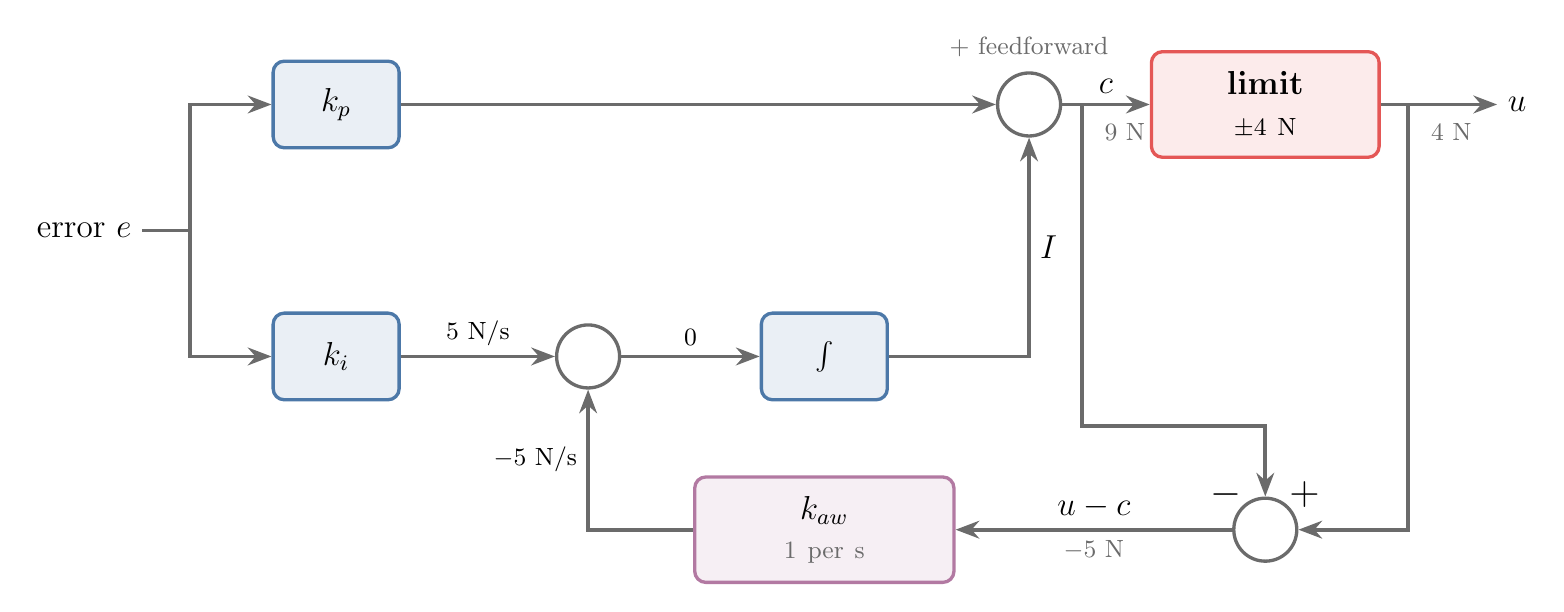
\begin{tikzpicture}[every node/.append style={font=\large}]
  \node (e) at (0,0) {error $e$};
  \node[box=cblue, minimum width=1.6cm] (kp) at (3.2,1.6) {$k_p$};
  \node[box=cblue, minimum width=1.6cm] (ki) at (3.2,-1.6) {$k_i$};
  \node[circle, draw=cgrey, fill=white, minimum size=0.8cm, inner sep=0pt] (add) at (6.4,-1.6) {};
  \node[box=cblue, minimum width=1.6cm] (int) at (9.4,-1.6) {$\int$};
  \node[circle, draw=cgrey, fill=white, minimum size=0.8cm, inner sep=0pt] (sum) at (12.0,1.6) {};
  \node[box=cred, text width=2.4cm] (lim) at (15.0,1.6) {\textbf{limit}\\[1pt] \small $\pm$4 N};
  \node (u) at (18.2,1.6) {$u$};
  \draw[arrow] (e.east) -- ++(0.6,0) |- (kp.west);
  \draw[arrow] (e.east) -- ++(0.6,0) |- (ki.west);
  \draw[arrow] (kp) -- (sum);
  \draw[arrow] (ki) -- node[above] {\small 5 N/s} (add);
  \draw[arrow] (add) -- node[above] {\small 0} (int);
  \draw[arrow] (int.east) -| node[pos=0.75, right] {$I$} (sum.south);
  \draw[arrow] (sum) -- node[above] {$c$} (lim);
  \node[font=\small, text=cgrey, anchor=north west] at ($(sum.east)+(0.4,-0.1)$) {9 N};
  \draw[arrow] (lim) -- (u);
  \node[font=\small, text=cgrey, anchor=north west] at ($(lim.east)+(0.5,-0.1)$) {4 N};
  \node[font=\small, text=cgrey, anchor=south] at ($(sum.north)+(0,0.05)$) {+ feedforward};
  % the extra feedback path: u - c through k_aw
  \node[circle, draw=cgrey, fill=white, minimum size=0.8cm, inner sep=0pt] (gap) at (15.0,-3.8) {};
  \node[box=cpurple, text width=2.8cm] (kaw) at (9.4,-3.8) {$k_{aw}$\\ \small\textcolor{cgrey}{1 per s}};
  \draw[arrow] ($(lim.east)+(0.35,0)$) |- (gap.east);
  \node[font=\Large] at ($(gap.north east)+(0.2,0.15)$) {$+$};
  \draw[arrow] ($(sum.east)+(0.25,0)$) |- node[pos=0.8, above] {} ($(gap.north)+(0,0.9)$) -- (gap.north);
  \node[font=\Large] at ($(gap.north west)+(-0.2,0.15)$) {$-$};
  \draw[arrow] (gap) -- node[above] {$u - c$} node[below, font=\small, text=cgrey] {$-$5 N} (kaw);
  \draw[arrow] (kaw.west) -| node[pos=0.75, left] {\small $-$5 N/s} (add.south);
\end{tikzpicture}
\end{document}
